\section{Buziness analyze : Bezint eer ge begint}

Het is heel belangrijk dat de business analist voldoende geëngageerde stakeholders heeft. Zij moeten immers hun expertise aan hem doorgeven. Zonder hun input kan er onmogelijk van een degelijke analyse gesproken worden en bovendien moeten die stakeholders voldoende geëngageerd zijn om in de analyse mee te gaan. Het is heel belangrijk dat de business analist een degelijke, kwalitatieve situatieanalyse maakt zodat de bedrijfsvoering goed begrepen is. Het spreekt vanzelf dat hij ook heel bedreven moet zijn in change management.

\textbf{De business analist staat in voor het uitvoeren van een accurate impact analyse en moet mogelijke implicaties inschatten.}

Een business analist heeft nood aan verschillende leiderschapskwaliteiten:

\begin{multicols}{2}
\begin{enumerate}
    \item Leadership of self
    \item Leadership within project
    \item Leadership within your organisation
    \item Leadership in the wider world
\end{enumerate}
\end{multicols}
%afbeelding nog plaatsen

\begin{center}
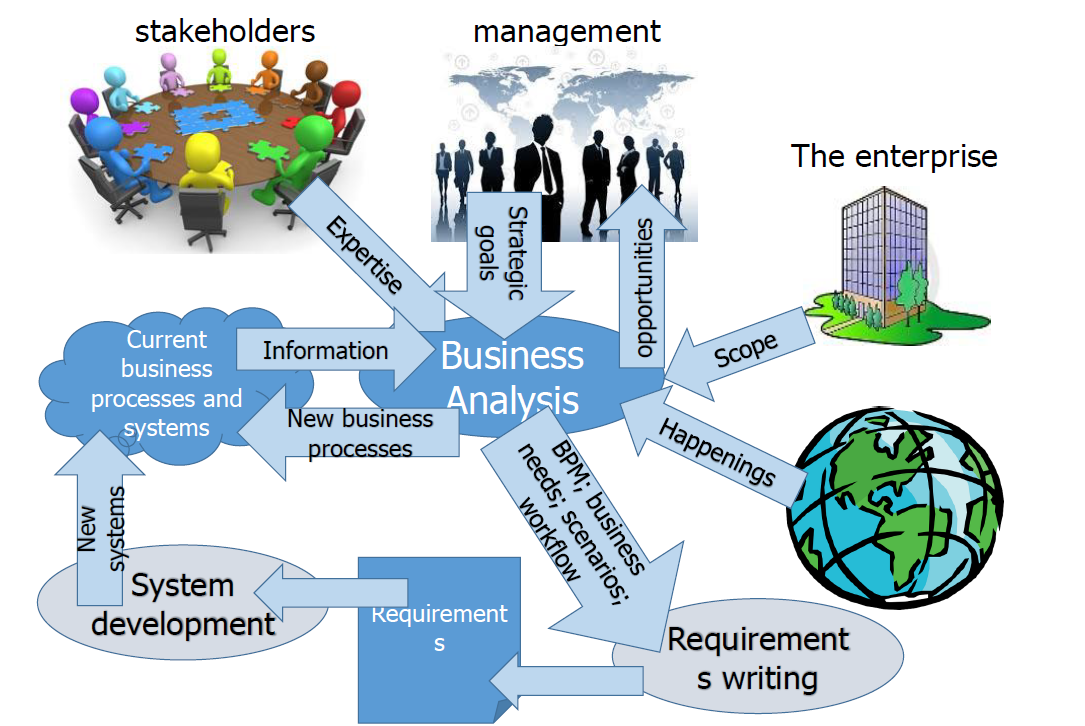
\includegraphics[width=4in]{img/stakeholders}%
\captionof{figure}{text}
\label{labelname}%
\end{center}

